\chapter{Needle Localization in MR Images}
\label{sec:mritracking} % Always give a unique label
% use \chaptermark{}
% to alter or adjust the chapter heading in the running head

\section{Software Architecture}
\subsection{Simulated MRI Scanner}
Full 3D MRI volumes take a long time to produce, especially if high resolution is desired: the scan time for each volume used in this thesis was approximately 5 minutes. This is a prohibitively long time in the context of real-time intraoperative imaging, so the MRI would be configured to provide 2D scans in requested planes with limited field of view. To simulate this functionality, a  Slicer module was created to resection 2D slices from each 3D volumes at specified depths.

\subsection{Needle Tracking Module}
A second Slicer module manages the needle tracking process. Figure \ref{fig:MRI_architecture} shows the architecture of this module relative to the Slicer environment and the needle modeling utility. A linear transform node is set to match the pose of the needle base in each saved volume. When commanded by the operator, the module requests slices of the MRI volume at evenly-spaced coordinates along the shaft of the needle. The thresholded image is grouped into contiguous regions, and the area and centroid are calculated for each region. The region with the centroid closest to the estimated position of the needle provided by the previous needle model curve is assumed to be the needle artifact, and the position of its centroid determines the observed position of the needle in this image. The position of the needle base is appended to this list of needle coordinates, and the combined list is used as one of the inputs for the needle curve optimization.

\begin{figure}[h]
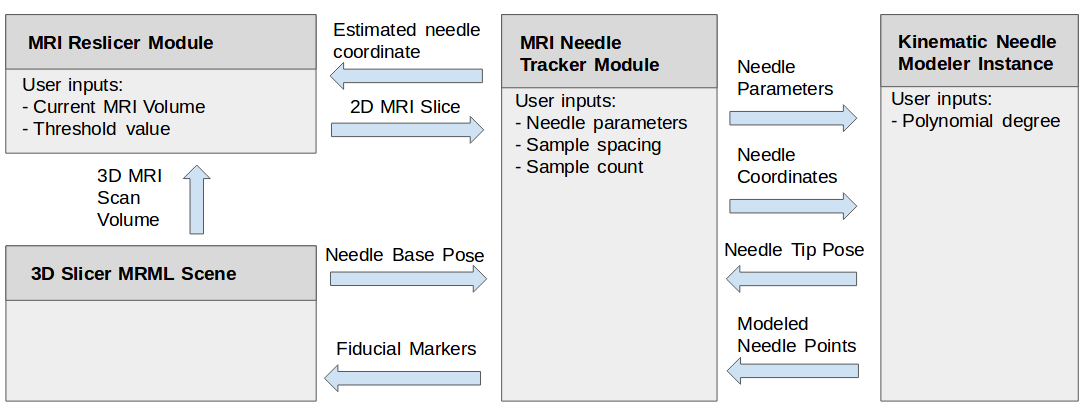
\includegraphics[width=1.0\textwidth]{Fig/chap5/MRI_software_architecture.png}
\caption{System architecture for needle detection and modeling from MRI data.}
\label{fig:MRI_architecture}
\end{figure}

\begin{figure}[h]
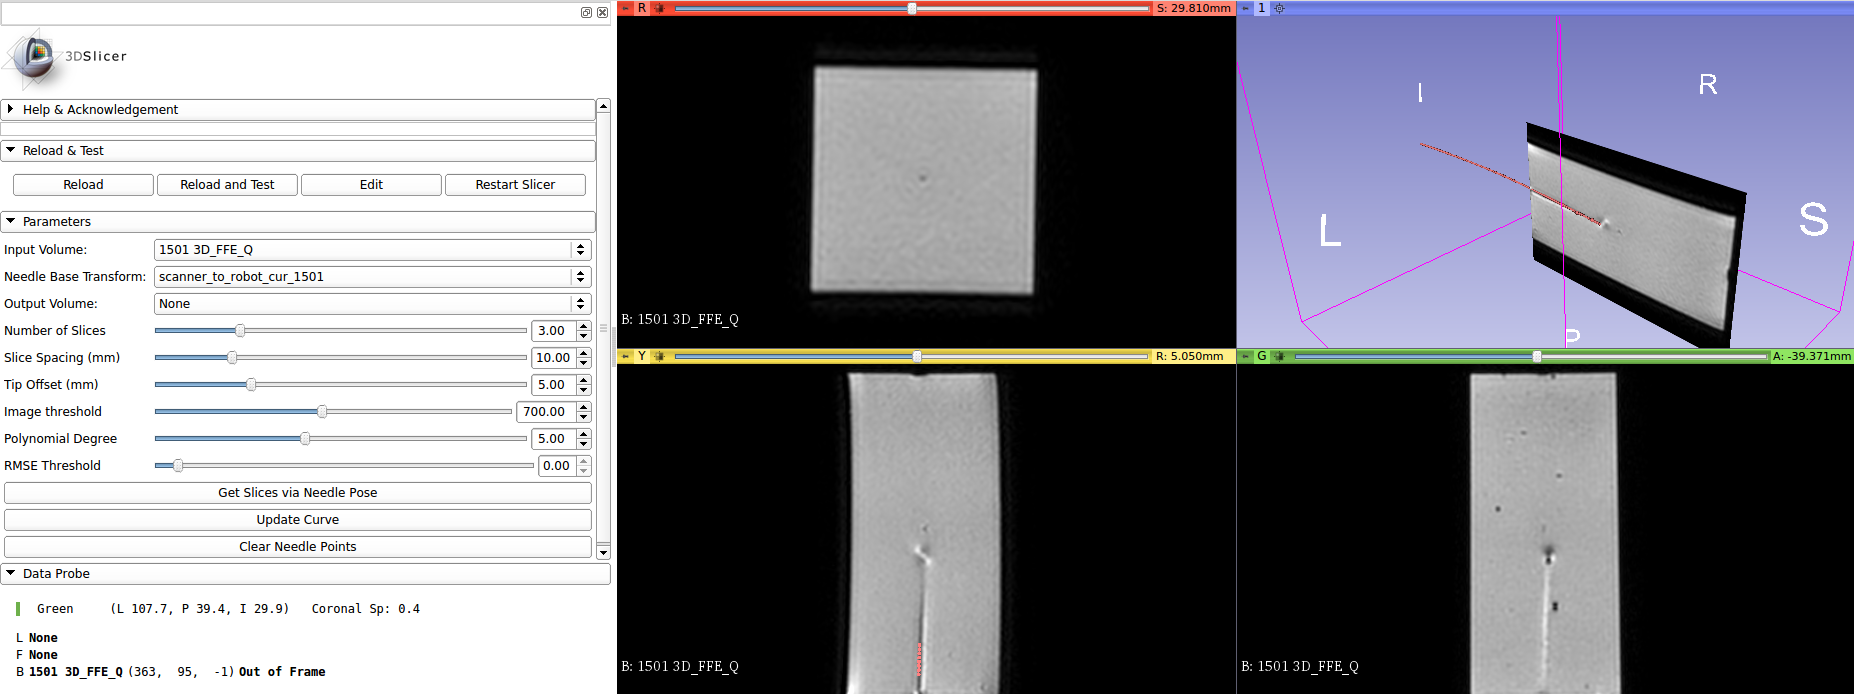
\includegraphics[width=1.0\textwidth]{Fig/chap5/MRINeedleTipTracker_module.png}
\caption{User interface for MRINeedleTipTracker 3D Slicer module.}
\label{fig:slicer_gui}
\end{figure}

\section{Experiment}

The purpose of this experiment is to validate the parametric curve fit and needle model on imagery representative of what would be available from intraoperative imagery during an MRI-guided insertion.

Several assumptions made to reduce the complexity of the experiment and facilitate needle tracking are listed below.

\begin{itemize}
\item A single beveled-tip clinical-style biopsy needle is to be inserted and tracked.
\item The initial vector of the needle is normal to the axial plane, and the actual pose of the needle base exactly matches the recorded pose.
\item Only homogeneous gelatin tissue phantoms are considered. The problem of identifying the needle in the presence of anatomy or other clutter is not addressed.
\item New MR data is acquired and transmitted instantaneously.
\end{itemize}

\subsection{MRI Data Collection}
The set of MRI volumes used in this experiment was captured in the 3T scanner at UMass Medical Center using a 3D Fast Field Echo protocol. The dimensions of each voxel are 0.4mm x 0.4mm x 0.5mm. The phantom used was made of agar gelatin. The needle was a 150mm stainless steel (E = 200 GPa) clinical-style biopsy needle with a beveled tip and a diameter of 2mm. Removable plastic spacers with a thickness of 5.95mm regulated the insertion distance. Two spacers were removed between scans, so the needle moves in increments of 11.9mm. Five scans were collected in total. The plastic alignment frame shown in Figure \ref{fig:needle_guide} kept the needle aligned along a known vector relative to the phantom. When used in conjunction the alignment frame and spacers allow the 6-DOF pose of the needle base to be calculated in each scan without the use of a Z-frame or external tracking equipment.

\begin{figure}[h]
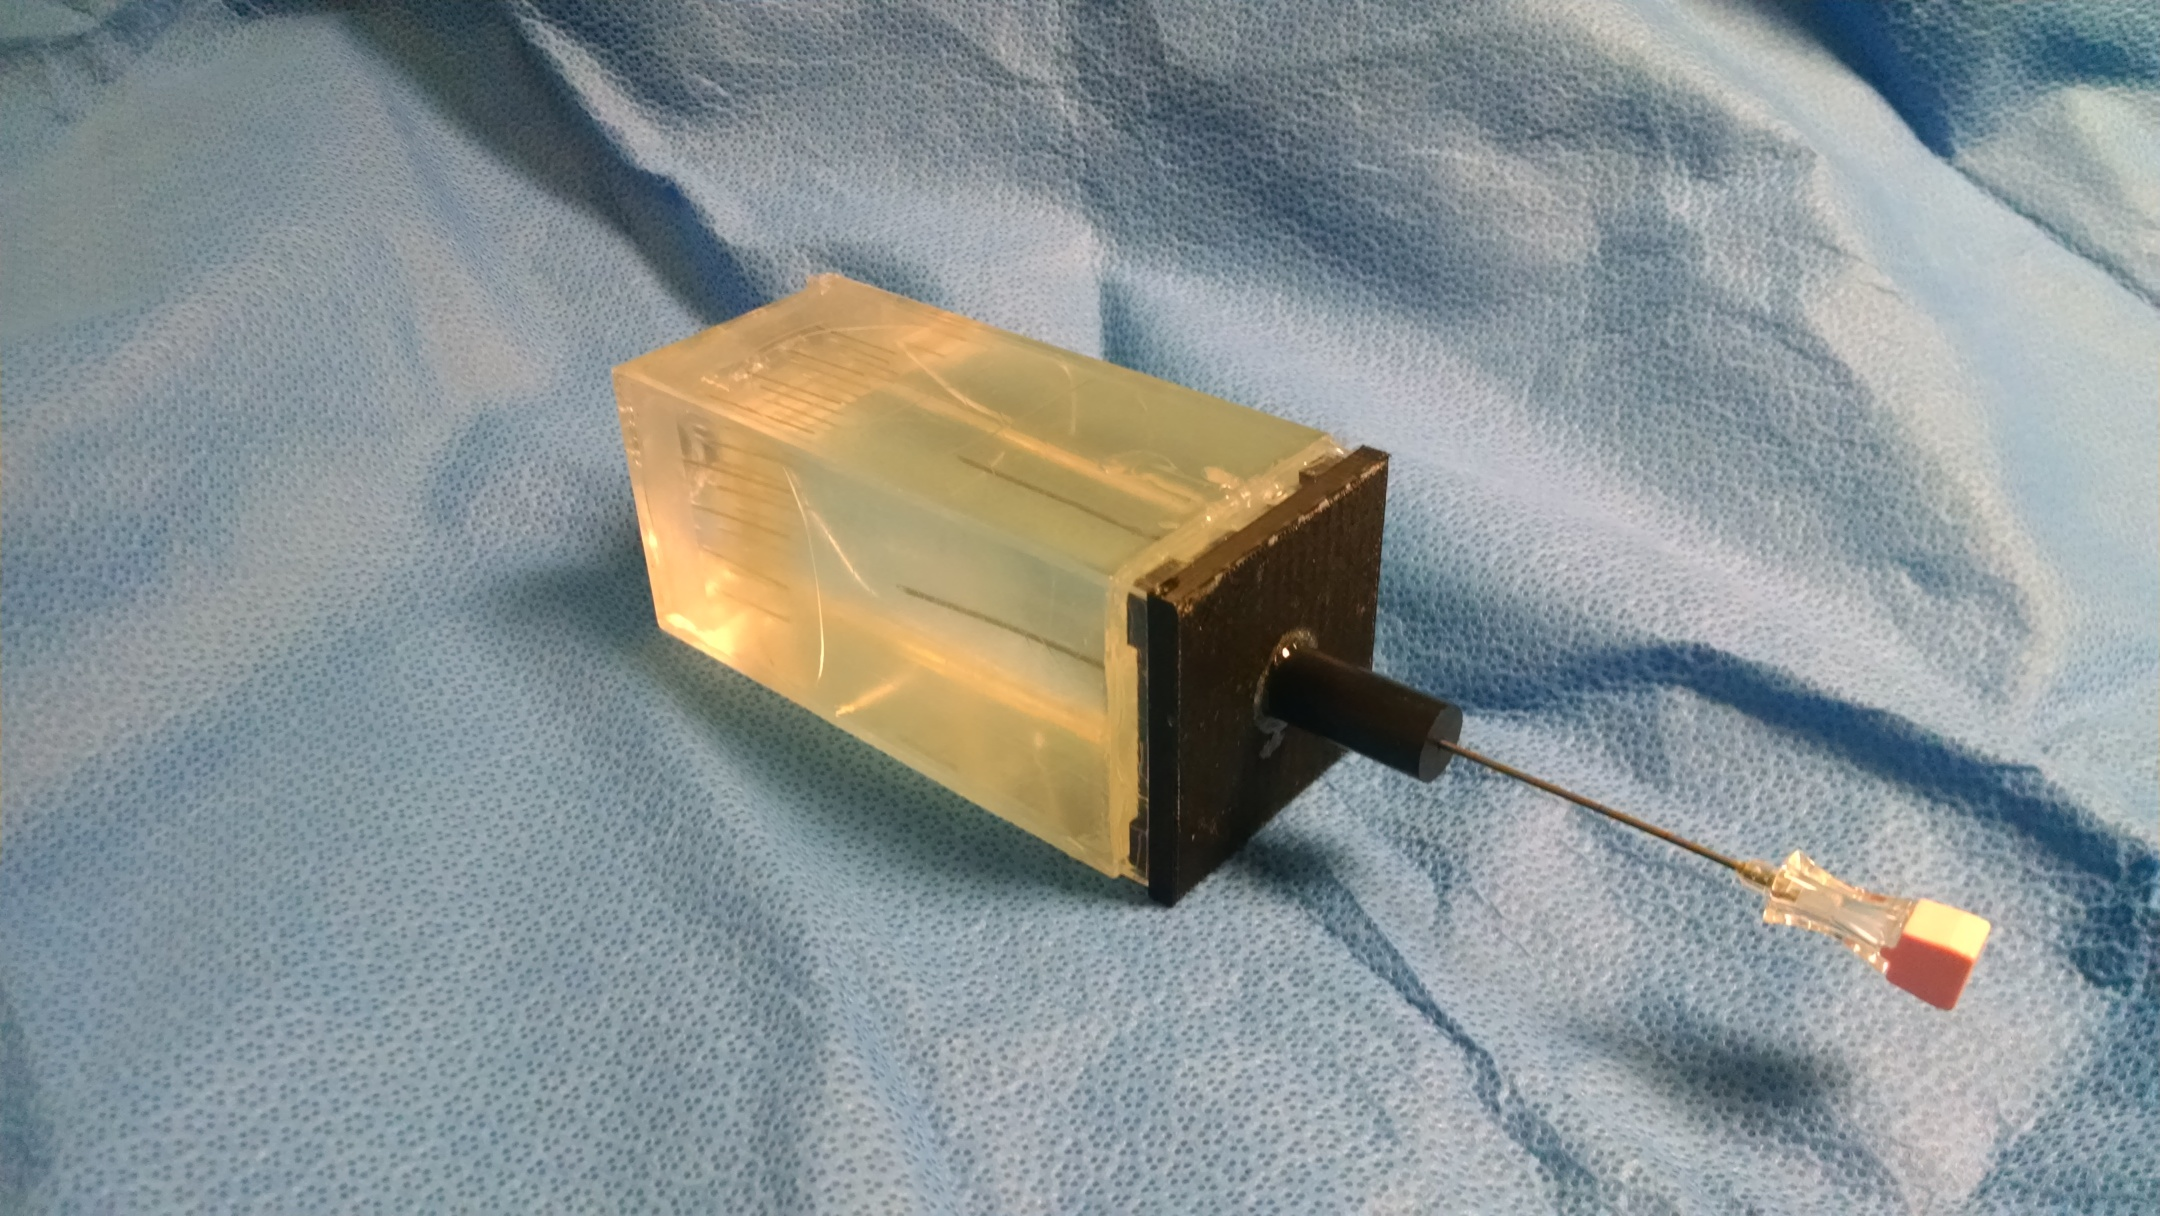
\includegraphics[width=1.0\textwidth]{Fig/chap5/phantom_with_needle_guide_small_2.jpg}
\caption{Tissue phantom with needle alignment frame and biopsy needle.}
\label{fig:needle_guide}
\end{figure}

\subsection{Needle Localization}

Each volume was thresholded at intensity 1500 to isolate the needle artifact. The segmentation labelmap was exported and processed separately.

The MRI volumes for each insertion step were loaded in sequence and a linear transform was set to match the pose of the needle base at each step. The needle localization algorithm was run on each dataset in turn to generate an array of points representing the simulated needle.

\section{Results}

% TODO: (Fu) "The model characterizes well the behavior of the needle with relatively small insertion distance (in Fig. 4.5, 4.6) and has a large error for large insertion depth, no matter the order of polynomial chosen, as noted in the discussion section. Is there any thought on how to improve the performance? If so, please include them in the discussion."

% TODO: (Fu) "Is it possible to compare the result with a dynamic model of the needle and vision-based state estimation?"

The baseline for the position of the needle shaft in the phantom was established by segmenting the needle artifact by intensity and computing the centroid of its cross section in every axial scan slice. Figure \ref{fig:seg_2001} shows the segmentation for the final step of the insertion, and Figure \ref{fig:ground_truth_2001} shows the positions of the centroids in successive axial planes. The error for each model is computed as the difference between the centroid coordinate and the modeled coordinate in each slice.

\begin{figure}[h]
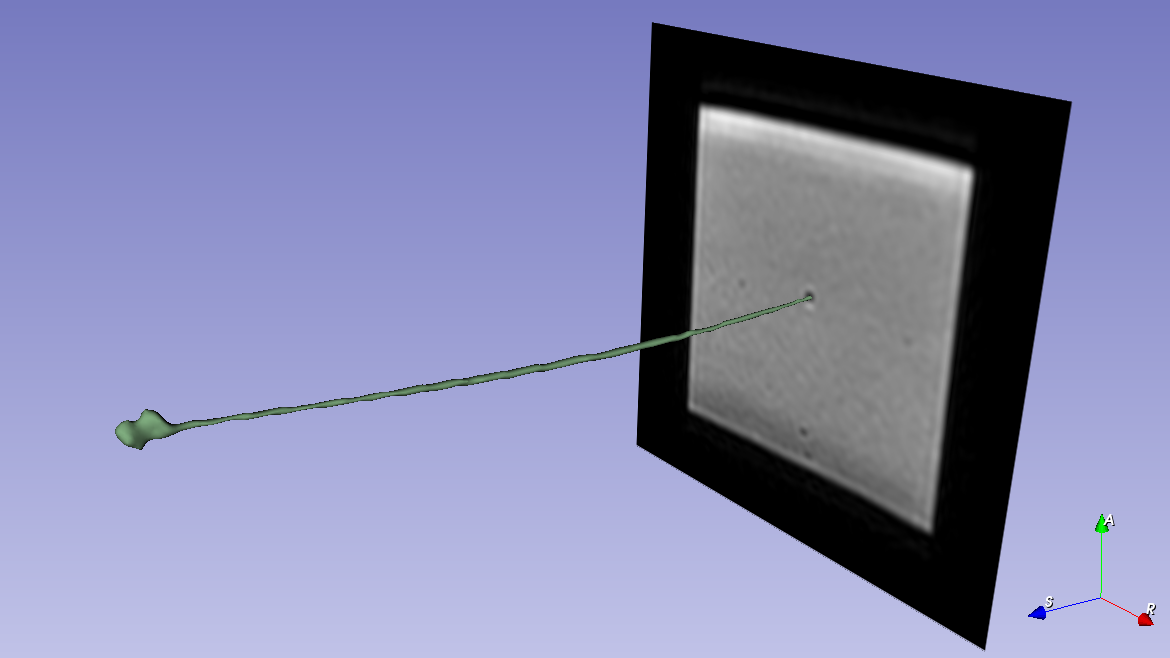
\includegraphics[width=1.0\textwidth]{Fig/chap5/segmented_artifact_2001.png}
\caption{Segmentation of needle artifact generated by thresholding MRI volume.}
\label{fig:seg_2001}
\end{figure}

\begin{figure}[h]
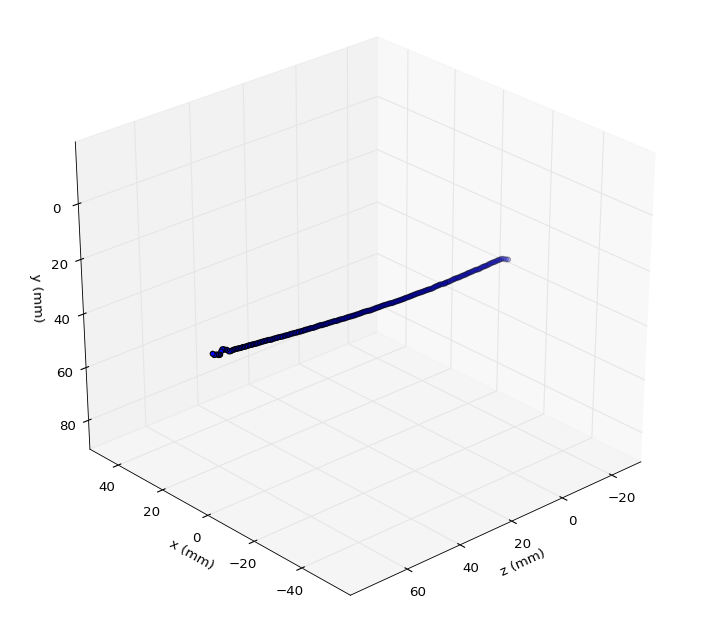
\includegraphics[width=1.0\textwidth]{Fig/chap5/neutral_axis_2001_b.png}
\caption{Baseline ground truth data, calculated from the centroids of the segmented artifact sectioned in the X-Y plane.}
\label{fig:ground_truth_2001}
\end{figure}

\subsection{Needle Localization at a Single Timestep}
\label{sec:mri_single_timestep}
At the start of curve optimization using data from an individual insertion step the needle is assumed to be a vector with magnitude matching the length of the needle. The sampling locations are offset from the estimated position of the needle tip by a user-configurable distance to avoid sampling points within the tip artifact.

Figure \ref{fig:results_error_comparison} shows the relative error using a 1st-, 3rd-, 5th-, and 7th-degree polynomials. The tip offset $\delta=5.0mm$, the sample spacing $d=26.0mm$, and the number of observed slices $k=3$. 

Figure \ref{fig:results_sample_comparison} show the effect on error relative to baseline as the number of slices observed over the length of the needle is increased. 

\begin{figure}[h]
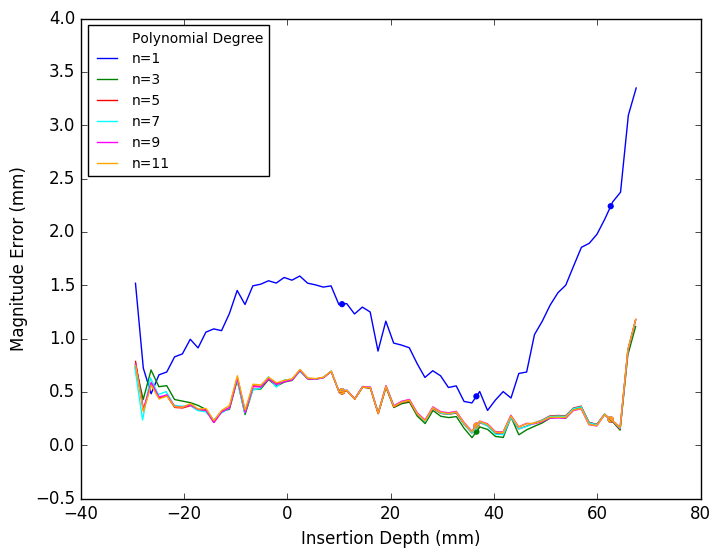
\includegraphics[width=1.0\textwidth]{Fig/chap5/errors_polynomials_3_samples.png}
\caption{Magnitude of in-plane error over insertion for various degrees of polynomial. Markers indicate the positions of the slices on the needle curve. $d=26.0mm$, $k=3$, $\delta=5.0mm$}
\label{fig:results_error_comparison}
\end{figure}

\begin{figure}[h]
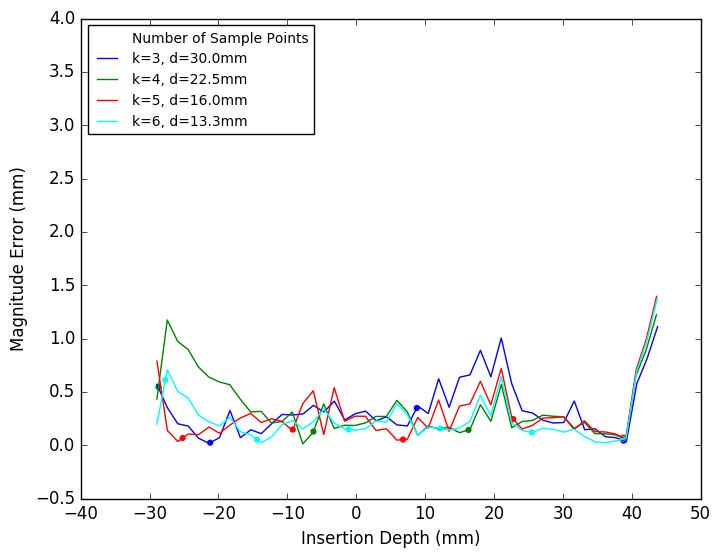
\includegraphics[width=1.0\textwidth]{Fig/chap5/errors_more_samples.png}
\caption{Magnitude of in-plane error over insertion for a variable number of sample points. $n=5$, $\delta=5.0mm$}
\label{fig:results_sample_comparison}
\end{figure}

\begin{figure}[h]

\includegraphics[width=1.0\textwidth]{Fig/placeholder.png}
\caption{Example polynomial curve fit plotted against the positions of the artifact centroids in transverse plane.}
\label{fig:curve_fit_artifact}
\end{figure}

\subsection{Needle Localization at Sequential Timesteps}
Needle tracking in a sequence of images consists of repeated application of the method for an individual timestep described in \ref{sec:mri_single_timestep}. The optimized curve from the previous localization step is used as the initial estimate for the next localization step. The curve was a 5th-degree polynomial. Three slice planes were selected, starting 5mm from the tip and spaced 10mm apart.

Figure \ref{fig:scan_slices} shows the positions of the scan planes and Figure \ref{fig:curve_points} shows points along the optimized curve for each insertion interval. Figure \ref{fig:curve_errors_fixed_spacing} shows the magnitude of error relative to the baseline for the optimized curve at each interval. Figure \ref{fig:curve_errors_variable_spacing} shows the magnitude of error when the spacing between the slices is increased as the needle is inserted.

\begin{figure}[h]
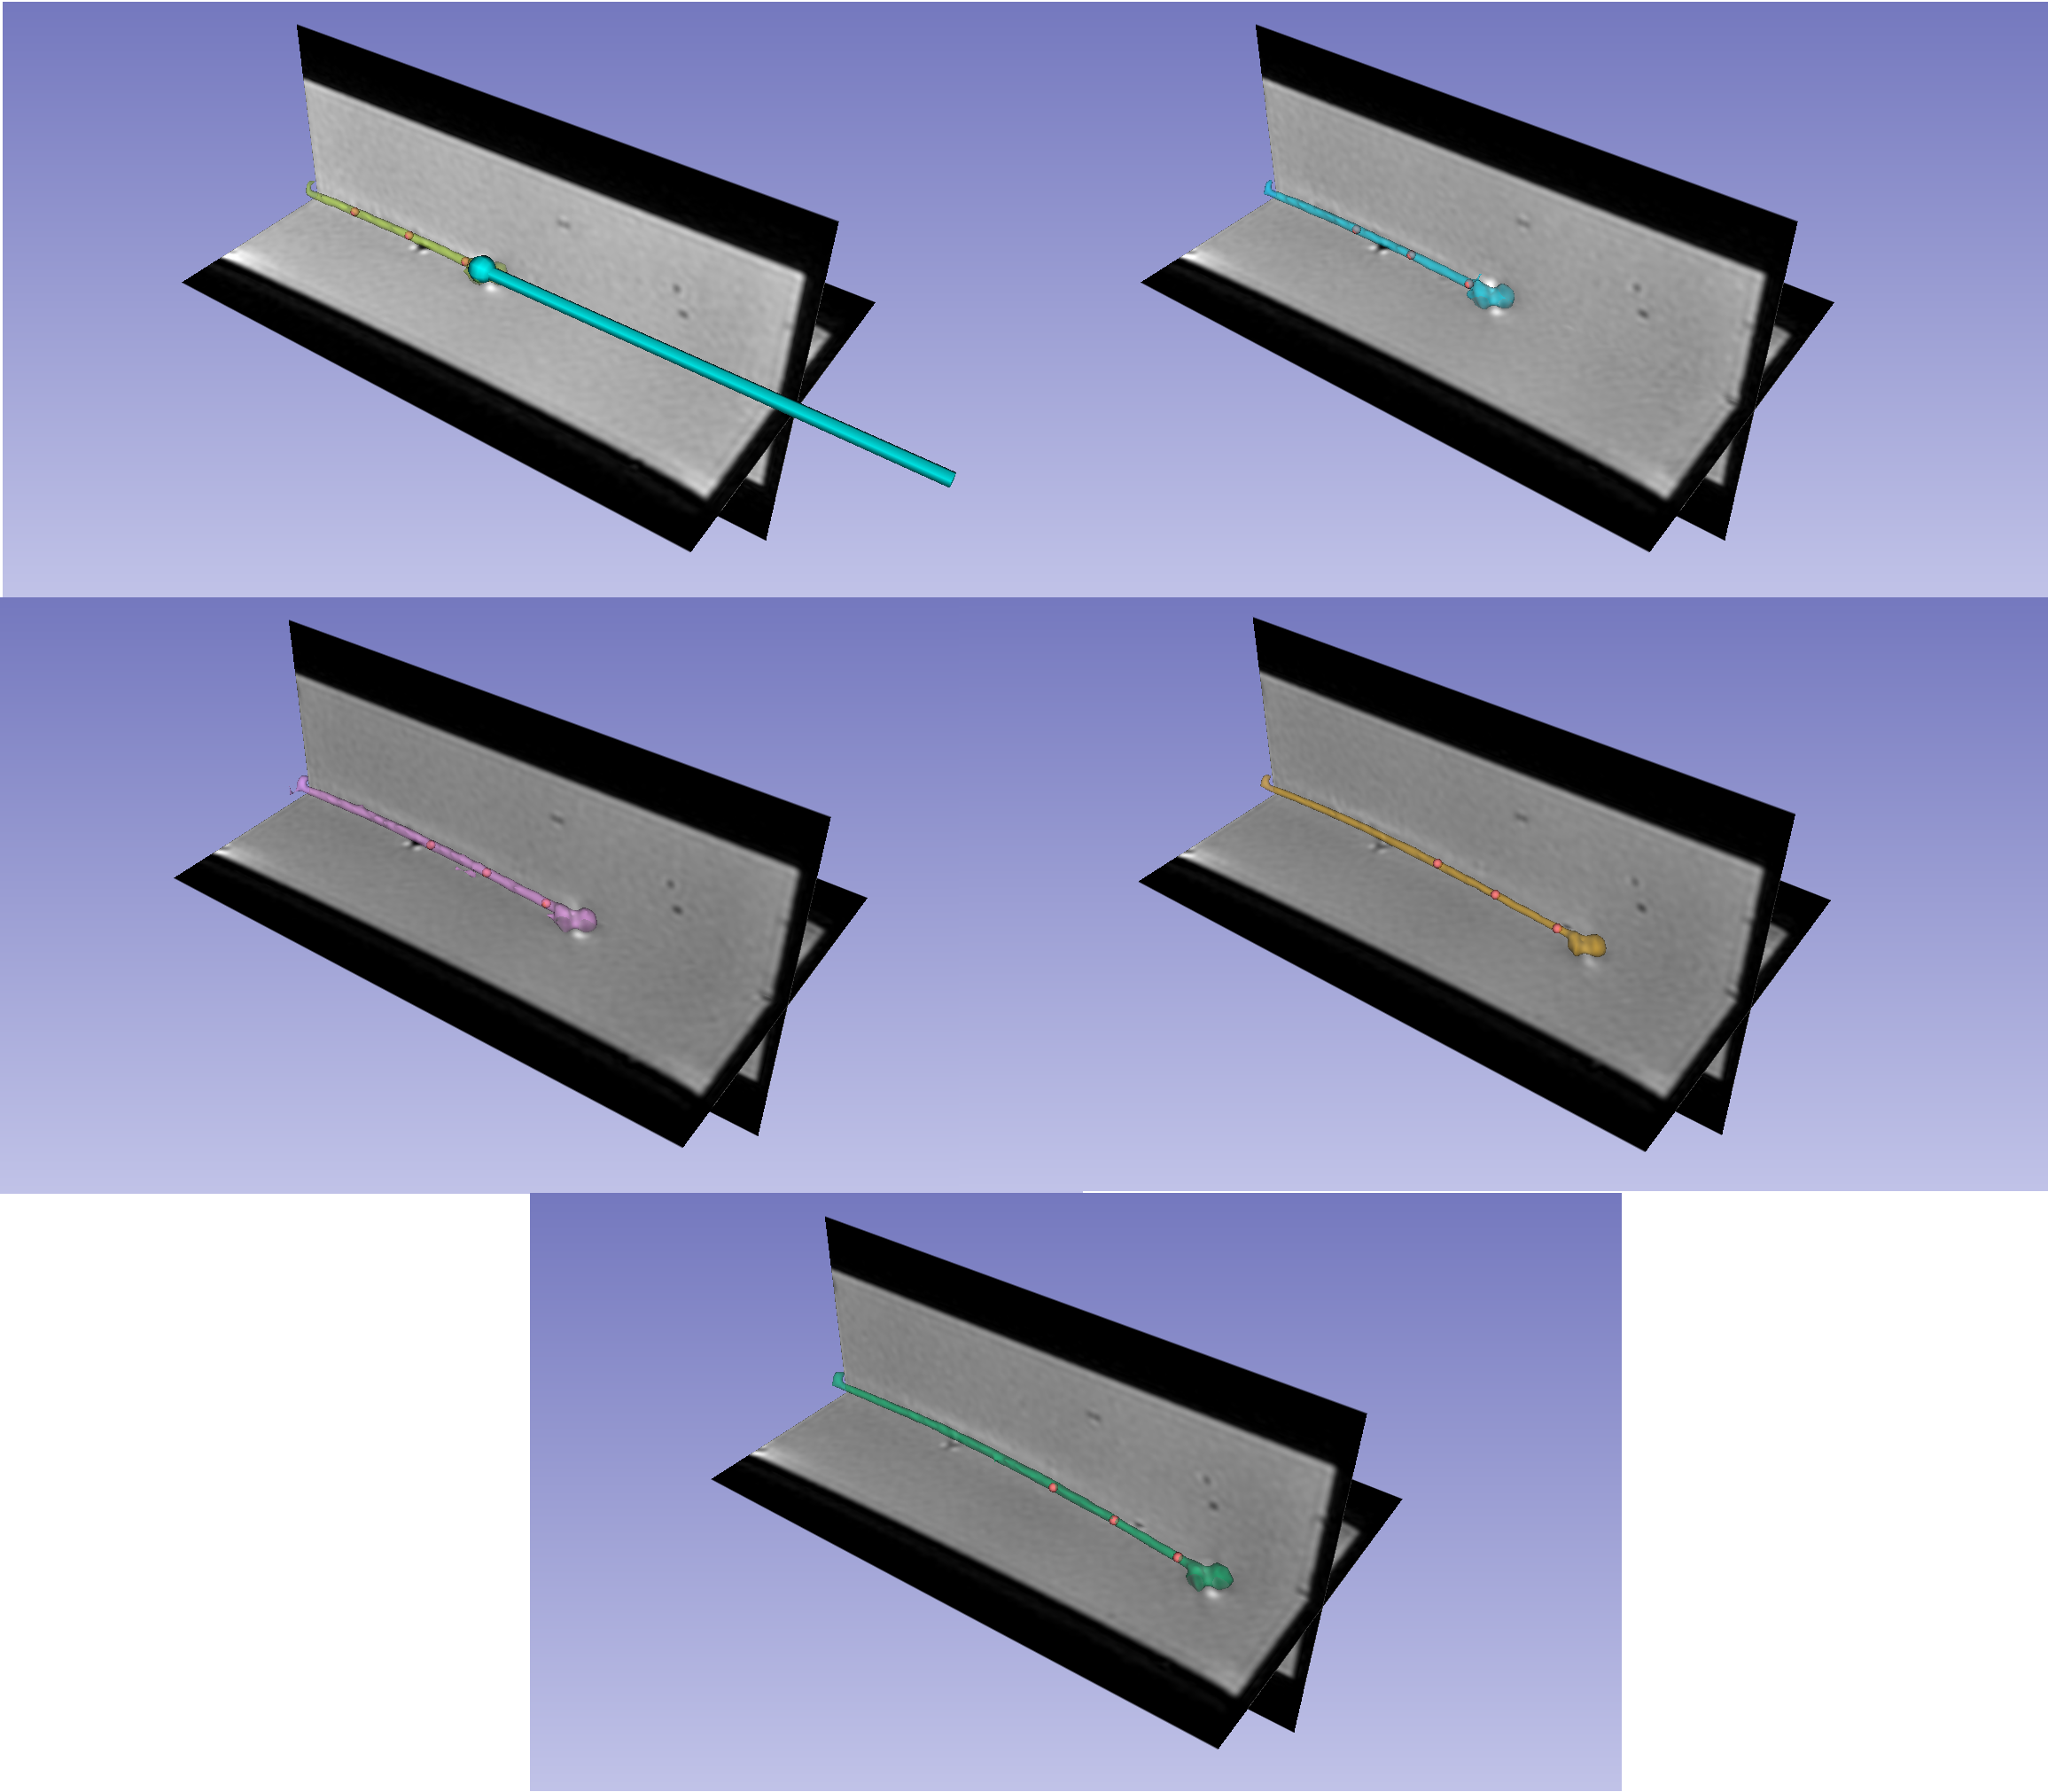
\includegraphics[width=1.0\textwidth]{Fig/chap5/scan_slices.png}
\caption{Positions of 2D scan planes at each insertion step, with segmented artifact.}
\label{fig:scan_slices}
\end{figure}

\begin{figure}[h]
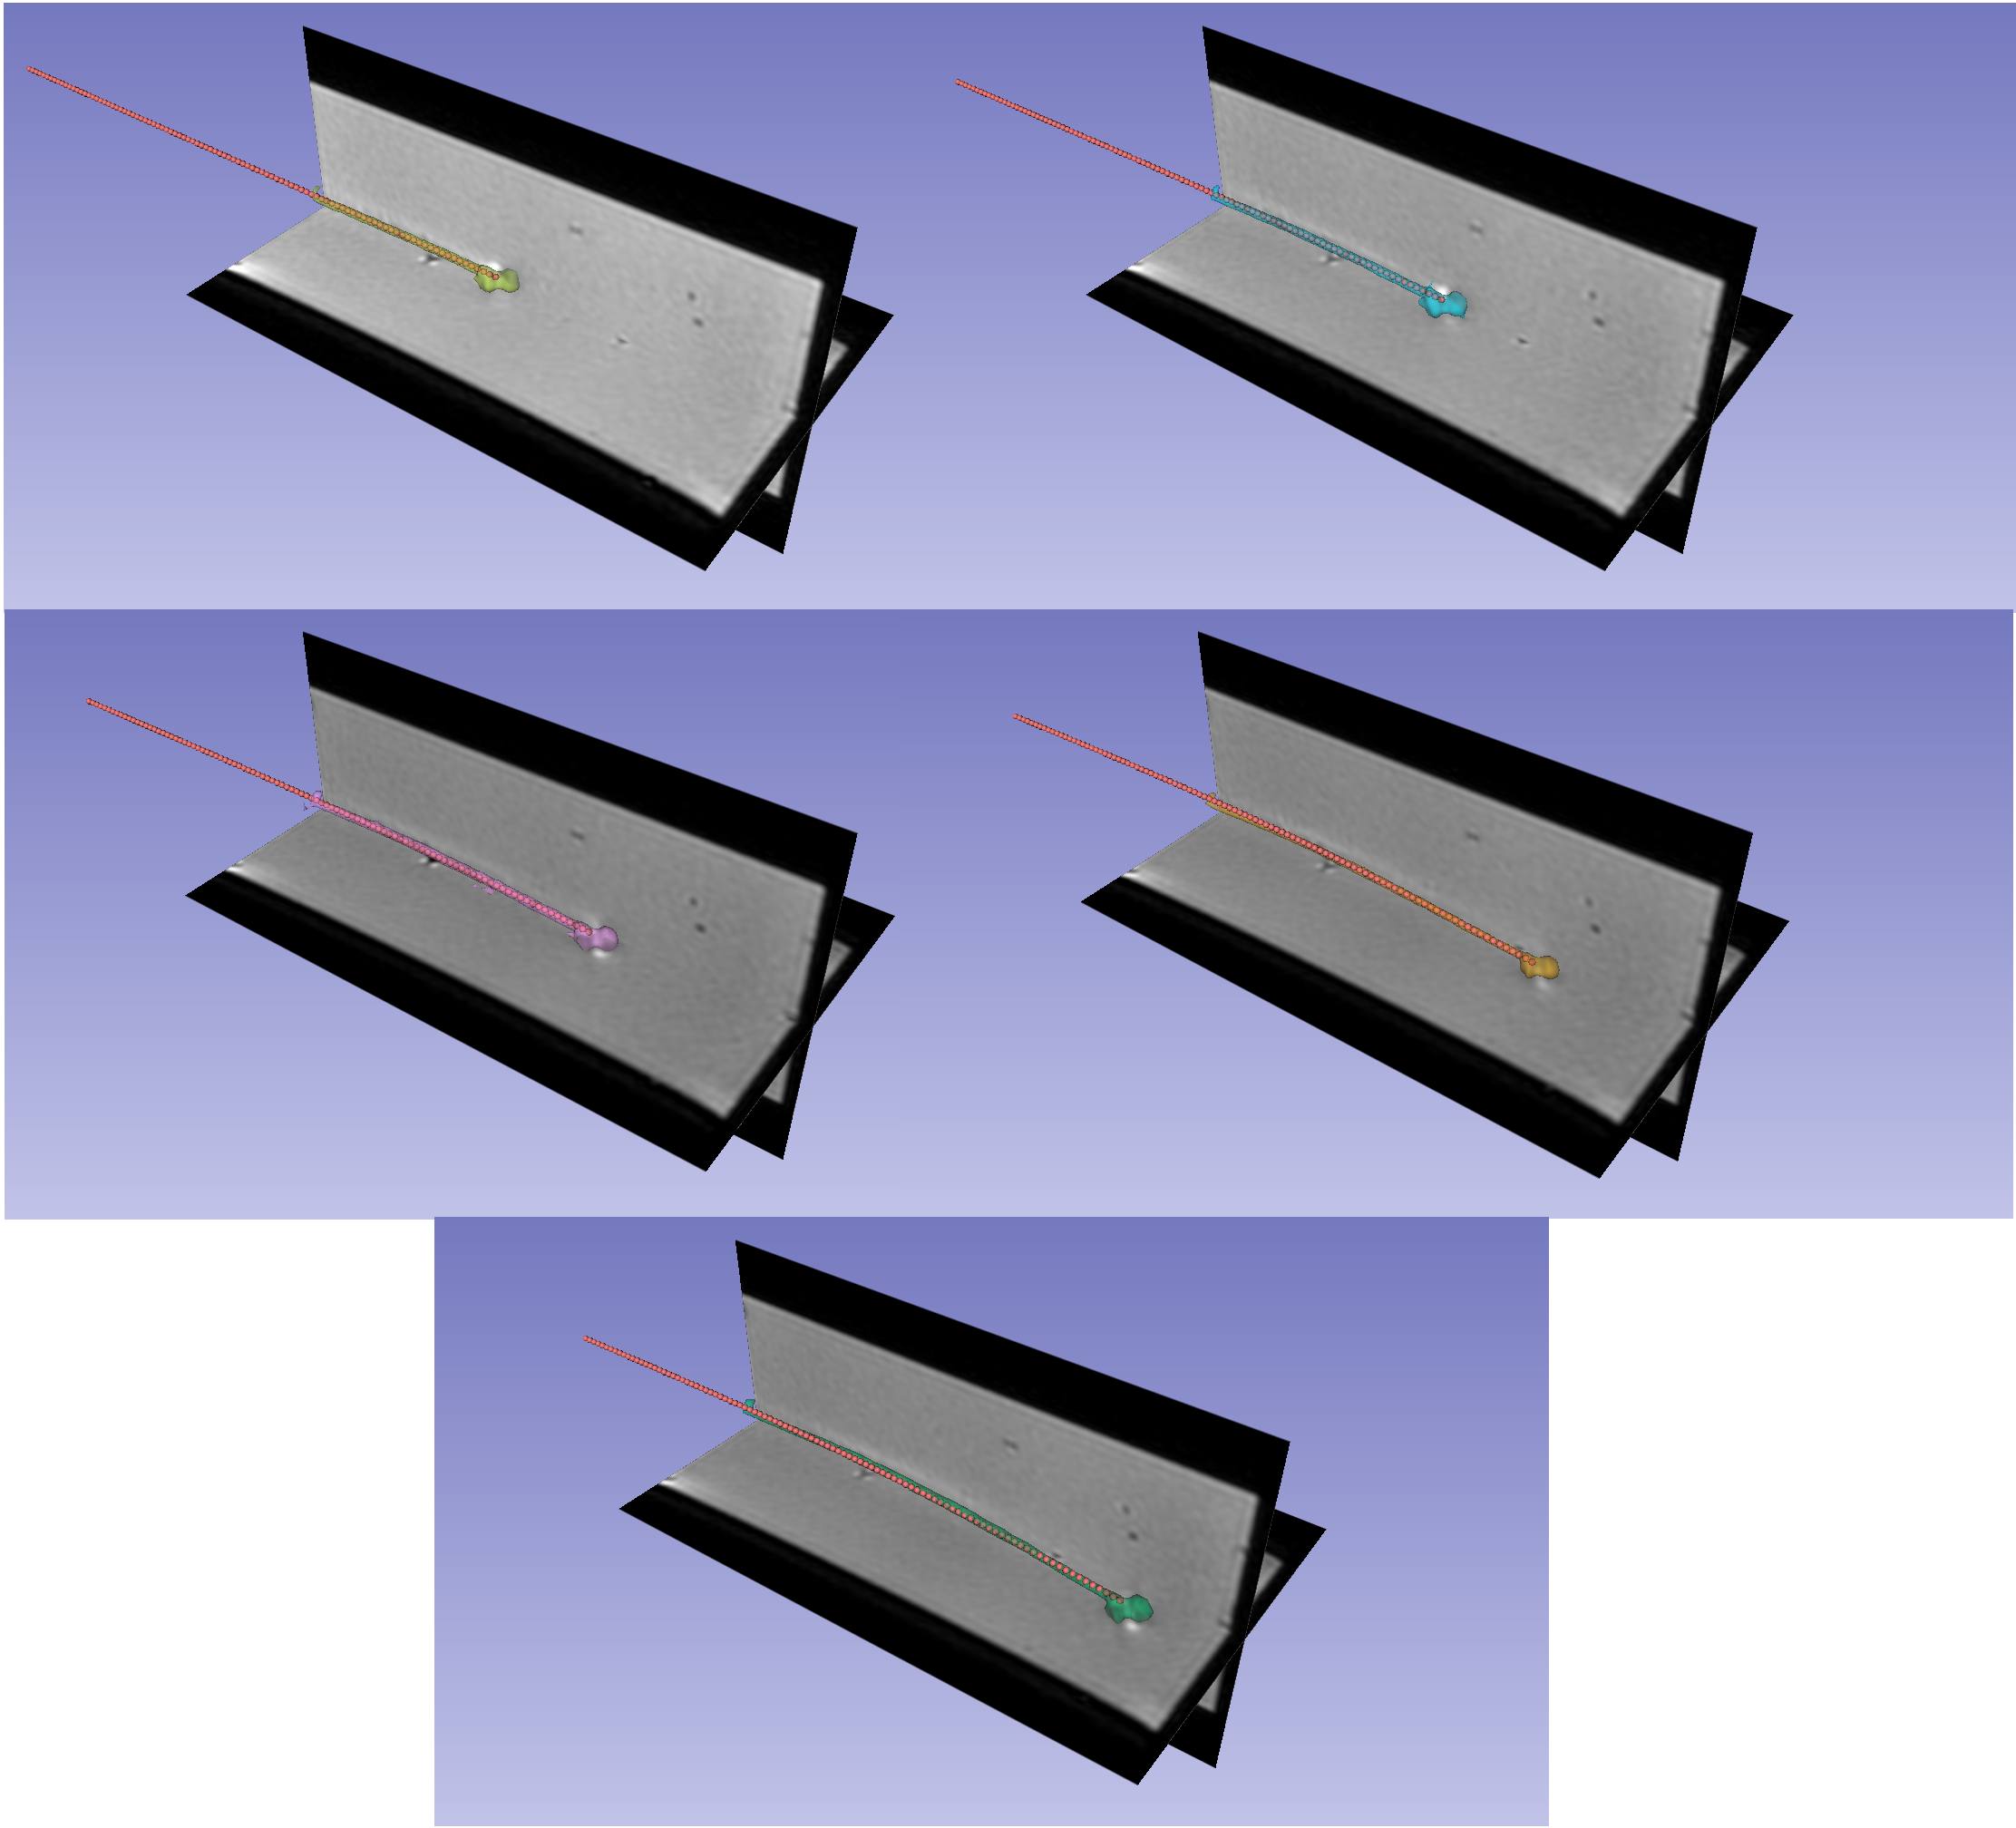
\includegraphics[width=1.0\textwidth]{Fig/chap5/insertions.png}
\caption{Modeled curve points at each insertion step, with segmented artifact.}
\label{fig:curve_points}
\end{figure}

\begin{figure}[h]
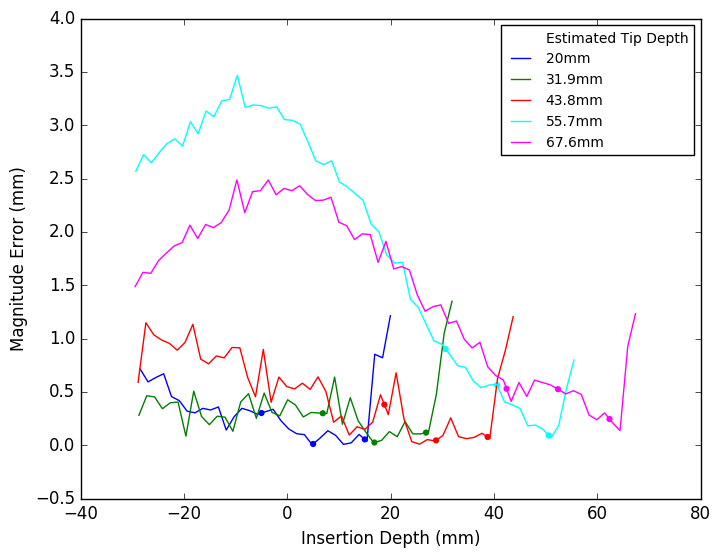
\includegraphics[width=1.0\textwidth]{Fig/chap5/error_curve_3_10.png}
\caption{Magnitude of error between the needle model and the artifact centroid.  $d=10mm$, $k=3$, $\delta=5mm$}
\label{fig:curve_errors_fixed_spacing}
\end{figure}

\begin{figure}[h]
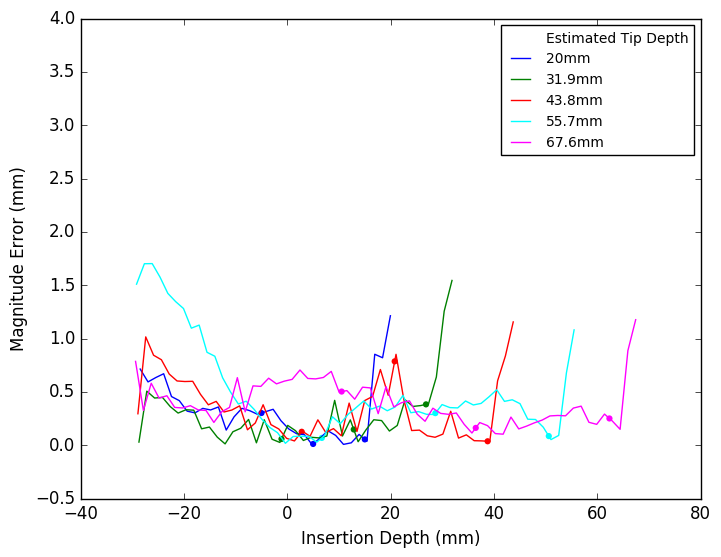
\includegraphics[width=1.0\textwidth]{Fig/chap5/error_curve_3_var.png}
\caption{Magnitude of error between the needle model and the artifact centroid, where the spacing between each slice increases with insertion depth.  $d=10mm + index_{step}*4mm$, $k=3$, $\delta=5mm$ }
\label{fig:curve_errors_variable_spacing}
\end{figure}


